

\chapter{IND-CCA secure Key Encapsulation from RSA}

    \section{Recap: The RSA Assumption}
        \begin{itemize}
            \item Recall that the RSA experiment $Exp-RSA_{\mathcal{A}}(\lambda)$ is defined as follows for a PPT adversary $\mathcal{A}$:
            \begin{itemize}
                \item Compute $(N,e,d) \leftarrow RSAGen(1^{\lambda})$, I.e. choose two random $\lambda$-bit primes $P$ and $Q$, set $N = P \cdot Q$ and $\Phi(N)=(P-1)\cdot(Q-1)$, 
                choose a random $e \leftarrow_{\$} \mathbb{Z}_N$ such that $gcd(e,\Phi(N))=1$ and compute a $d$ such that $e \cdot d \equiv 1 \ mod \ \Phi(N)$
                \item Choose a random $r \leftarrow_{\$} \mathbb{Z}_N$ and set $c \leftarrow r^e \ mod \ N$
                \item Compute $r' \leftarrow \mathcal{A}(N,e,c)$
                \item If ${r'}^e \equiv c\ mod\ N$ output 1, otherwise 0 $({r'}^e = r^e \Leftrightarrow r' = r)$
            \end{itemize}
            \item The RSA-assumption conjectures that it holds for every PPT-adversary $\mathcal{A}$ that 
            $$Pr[Exp-RSA_{\mathcal{A}}(\lambda)=1] \leq negl(\lambda)$$
        \end{itemize}
    
    \section{An RSA-based Key Encapsulation Mechanism}
        Let $RSAGen$ be an algorithm that generates RSA parameters and let $H: \mathbb{Z}_N \rightarrow \{0,1\}^{\lambda}$ be a hash function.
        The key-encapsulation mechanism $(KeyGen,Encaps,Decaps)$ is given as follows.
        \begin{itemize}
            \item $KeyGen(1^{\lambda})$: $(N,e,d) \leftarrow RSAGen(1^{\lambda})$, output $pk \leftarrow (N,e)$ and $sk \leftarrow (N,d)$
            \item $Encaps(pk=(N,e))$: Choose $r \leftarrow_{\$} \mathbb{Z}_N$ and compute $c \leftarrow r^e\ mod\ N$.
            Output $c$ and $K \leftarrow H(r)$.
            \item $Decaps(sk=(N,d),c)$: Compute and output $K \leftarrow H(c^d \ mod\ N)$
        \end{itemize}
    
    \section{$IND-CCA$ Security}
        \begin{theorem}\label{thm8.3}\ 
            \begin{itemize}
                \item Assume that the RSA assumption holds
                \item Assume further that $H$ is modeled as a random oracle
                \item Then $(KeyGen,Encaps,Decaps)$ is an IND-CCA secure key encapsulation mechanism
            \end{itemize}
        \end{theorem}
        \begin{proof}
            Assume towards contradiction that $\mathcal{A}$ is a PPT-adversary which breaks IND-CCA security of KEM with non-negligible advantage $\epsilon$.
            \begin{center}
	            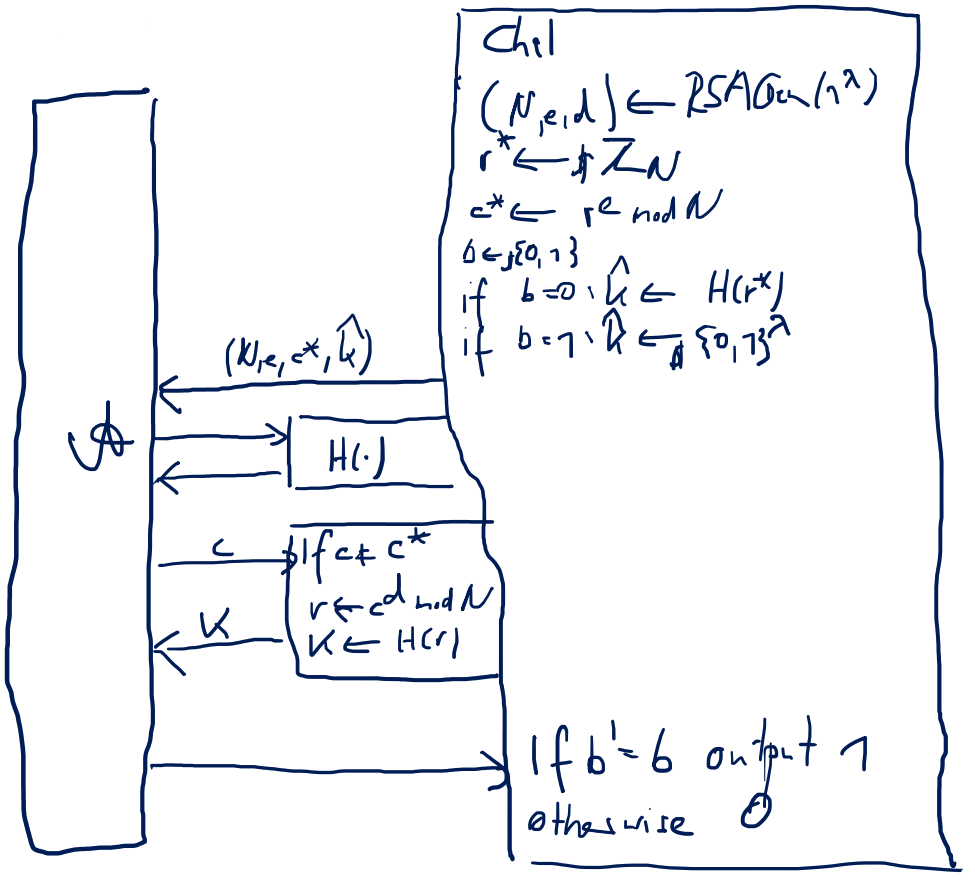
\includegraphics[width=160mm]{Graphics/IND-CCA secure Key Encapsulation from RSA/bla1.png}
            \end{center}
            Let $Query$ be the event that $\mathcal{A}$ queries $H$ with the value $r^*$.\\
            Conditioned on $\overline{Query}$, it holds that $H(r^*)$ is distributed uniformly (and independent) from the view of $\mathcal{A}$.
            This means $Pr[IND-CCA_{\mathcal{A}(\lambda)}=1 \mid \overline{Query}] = \frac{1}{2}$. It holds that
            \begin{align*}
                \frac{1}{2} + \epsilon \leq Pr[IND-CCA_{\mathcal{A}(\lambda)}=1] &= \underbrace{Pr[IND-CCA_{\mathcal{A}(\lambda)}=1 \mid \overline{Query}]}_{= \frac{1}{2}} 
                \cdot \underbrace{Pr[\overline{Query}]}_{\leq 1}\\
                &+ \underbrace{Pr[IND-CCA_{\mathcal{A}(\lambda)}=1 \mid Query]}_{\leq 1} \cdot Pr[Query] \leq \frac{1}{2} + Pr[Query]
            \end{align*}
            $\Rightarrow$ $Pr[Query] \geq \epsilon$\\
            We will now construct an adversary $\mathcal{A}'$ which breaks the RSA-assumption with probability $\epsilon$.
            \begin{center}
	            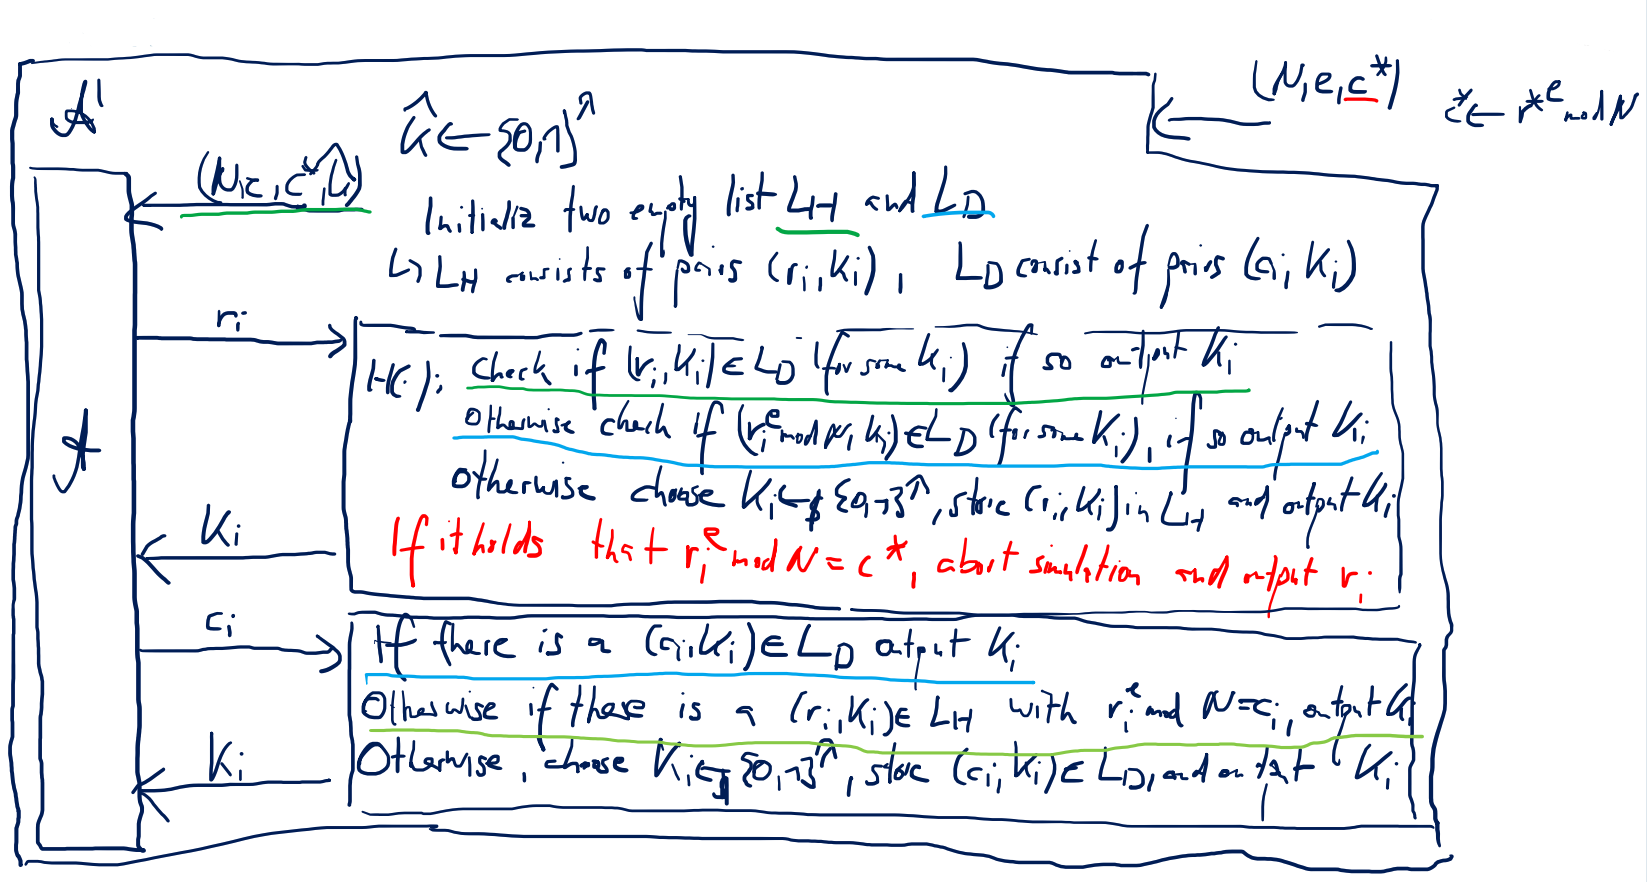
\includegraphics[width=160mm]{Graphics/IND-CCA secure Key Encapsulation from RSA/bla2.png}
            \end{center}
            From the view of $\mathcal{A}$, $\mathcal{A}'$ simulates the IND-CCA experiment faithfully.
            Moreover, $\mathcal{A}'$ wins the RSA experiment, if and only if $Query$ happens.
            It follows
            $$Pr[Expp-RSA_{\mathcal{A}'}(\lambda)=1] = Pr[Query] \geq \epsilon$$
            which is non-negligible.\\
            $\Rightarrow$ $\mathcal{A}'$ breaks the RSA problem with non-negligible probability!\\
            $\Rightarrow$ Contradiction to the RSA assumption.
        \end{proof}

    \section{Summary}
        \begin{itemize}
            \item We can construct an IND-CCA secure key encapsulation mechanism from the RSA assumption
            \item Recipe: Textbook RSA with random message and hashing
            \item Need to model hash function as a random oracle in the proof
        \end{itemize}


